\chapter{Практическая часть}
\label{cha:pract}

\section{Постановка задачи}

В рамках практической части работы, было выделены следующие задачи:

\begin{itemize}
 \item изучить средства разработки программного обеспечения для микрокотроллеров семейства ARM;
 \item адаптировать существующее открытое программное обеспечение к другой аппаратной платформе;
 \item создать работающие прототипы конечных устройств с трансиверами LoRa;
\end{itemize}

\section{Выбор аппаратной платформы}

\subsection{STM32L476G-Discovery}

Для разработки конечных устройств была выбрана отладочная плата STM32L476G-Discovery на базе 32-битного микроконтроллера STM32L476VGT6 с ядром ARM-Cortex M4.
Данный микроконтроллер является представителем семейства микроконтроллеров с низким энергопотреблением STM32L4 фирмы ARM.
Микроконтроллер имеет:
\begin{itemize}
 \item 3 устройства I2C;
 \item 3 устройства SPI;
 \item поддержка шины CAN;
 \item SWPMI;
 \item 2 x SAI;
 \item 12-битное ЦАП;
 \item драйвер LCD;
 \item 128 Кбайт SRAM;
 \item 1 МБайт Flash;
 \item Quad-SPI;
 \item touch sensing;
 \item USB OTG FS;
 \item поддержка JTAG отладки;
\end{itemize}

Удобство данной отладочной платы заключается в том, что вся необходимая вспомогательная периферия уже находится на плате, и подключена ко входам и выходам микроконтроллера.
В качестве вспомогательной периферии служат:

\begin{itemize}
 \item программатор/отладчик ST-LINK/V2-1;
 \item LCD дисплей;
 \item кнопка RESET;
 \item джойстик;
 \item встроенный амперметр, для измерения тока потребления микроконтроллера в режиме low power;
 \item USB OTG FS;
 \item аудио ЦАП;
 \item MEMS (микрофон, 3-осевой гироскоп, 6-осевой компас);
 \item Quad-SPI Flash память;
 \item светодиоды.
\end{itemize}

Вид на плату сверху отображён на рисунке \ref{fig:discovery}.

\begin{figure}[!h]
  \centering
  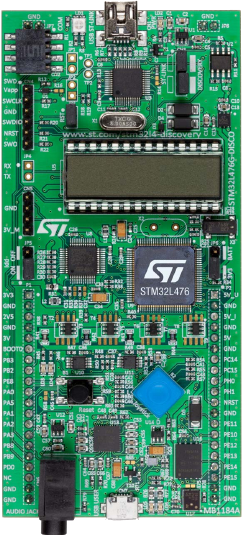
\includegraphics[height=0.3\textheight]{inc/img/discovery}
  \caption{Отладочная плата STM32L476G-Discovery}
  \label{fig:discovery}
\end{figure}

\subsection{Трансивер LoRa}

Модули Semtech LoRa представляют собой ВЧ-трансиверы, с возможностью создания 
топологии M2M (машина-машина) и ``звезда из здвёзд'' (сети LoRa). 
Эти устройства оптимизируют потребление энергии, увеличивая срок службы батарей 
конечных устройств.
Они подробно задокументированы, что делает процесс подключения к интерфейсу
 доступным для широкого круга разработчиков программно-аппаратного обеспечения 
инфраструктуры Интернета вещей.

Серия SX1272/78 имеют бюджет канала в -148 dBm. 
Высокая чувствительность в сочетании с усилителем LNA (малошумящий усилитель)
 +20 дБм обеспечивают надёжную связь для применения в промышленности 
\cite{Rizzi2017}.

\begin{table}[ht]
 \caption{Рабочие частоты для SX1272 и SX1278}
 \begin{tabular}{|c|c|c|}
  \hline
  Устройство & \begin{tabular}[c]{@{}c@{}}Минимальная\\ частота 
  (МГц)\end{tabular} & \begin{tabular}[c]{@{}c@{}}Максимальная\\ частота 
  (МГц)\end{tabular} \\ \hline
  SX1272     & 860                                                               
  & 1020                                                                 \\ 
  \hline
  SX1278     & 137                                                               
  & 525                                                                  \\ 
  \hline
\end{tabular}
 \label{tab:sx127x}
\end{table}

Чувствительность приёмника определяет минимальное значение мощности, которое 
требуется ему для демодуляции и декодирования с целью достижения определенной 
скорости передачи данных. 
Чувствительность обычно выражается в дБм и чем ниже значение, тем лучшую 
чувствительность имеет приёмник, поэтому, исходя из таблицы 
\ref{tab:sx127xParams} можно сделать вывод, что SX1278 имеет большую 
чувствительность приёмника перед SX1272.

\begin{table}[ht]
 \caption{Основные параметры приёмопередатчиков LoRa}
 \begin{tabular}{|c|c|c|c|c|}
\hline
\multirow{2}{*}{\begin{tabular}[c]{@{}c@{}}Приёмо-\\ передатчик\end{tabular}} & 
\multicolumn{4}{c|}{Параметры LoRa}                                              
                                                                                 
                                                                                 
                                                          \\ \cline{2-5} 
                                                                              & 
\begin{tabular}[c]{@{}c@{}}SF \\ диапазон\end{tabular} & 
\begin{tabular}[c]{@{}c@{}}Ширина\\  полосы\\ частот (КГц)\end{tabular} & 
\begin{tabular}[c]{@{}c@{}}Эффективная \\ скорость\\ передачи \\ данных\\ 
(кбит/с)\end{tabular} & \begin{tabular}[c]{@{}c@{}}Чувстви-\\ тельность\\ 
(дБм)\end{tabular} \\ \hline
SX1272                                                                        & 
6..12                                                  & от 125 до 500           
                                                & 0,24..37,5                     
                                                                 & -117..-137    
                                                          \\ \hline
SX1278                                                                        & 
6..12                                                  & от 7,8 до 500           
                                                & 0,018..37,5                    
                                                                 & -111..-148    
                                                          \\ \hline
\end{tabular}
 \label{tab:sx127xParams}
\end{table}

Был выбран приёмопередатчик Semtech SX1278. Выбор был обусловлен тем, что он 
уже имелся в наличии и его внутренняя структура схожа с трансивером SX1272 (они 
имеют общее руководство по эксплуатации).
Данный трансивер будет пригоден для исследовательских работ, но следует иметь в 
виду что для коммерческого использования в России следует выбрать трансивер 
SX1272, поскольку частоты около 868 МГц находятся в пределах поддерживаемых 
частот данного трансивера.

\begin{figure}[!h]
  \centering
  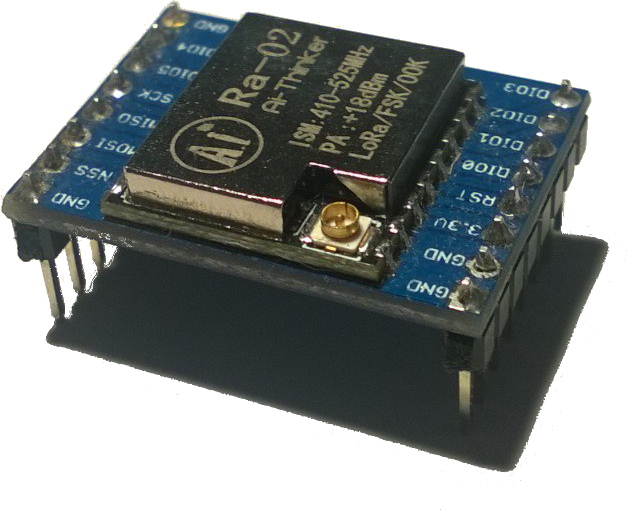
\includegraphics[height=0.3\textheight]{inc/img/SX1278}
  \caption{Трансивер SX1278}
  \label{fig:sx1278}
\end{figure}

Внутренние регистры трансиверов доступны через интерфейс связи SPI.
SPI ""--- это синхронный последовательный полнодуплексный протокол передачи 
данных. 
Обмен по протоколу SPI осуществляют ведущее (\textit{Master}) и подчинённое 
(\textit{Slave}) устройство, приём передачу данных инициирует именно ведущее.

Этот протокол использует 4 линии для связи, которые описываются как:
\begin{itemize}
 \item \textbf{SCLK}. Соответствует тактовому сигналу, генерируется ведущим и 
синхронизирует передачу данных;
 \item \textbf{MOSI} (\textit{Master Out Slave In}). Передача основных данных 
от ведущего к подчиненному устройству;
 \item \textbf{MISO} (\textit{Master In Slave Out}). Передача основных данных 
от подчиненного к ведущему устройству устройству;
 \item $\overline{\text{\textbf{NSS}}}$ (\textit{Slave Select}). Выборка 
%подчиненного устройства. Используется для связи нескольких подчиненных 
%устройств к ведущему. 
\end{itemize}

Радиомодули LoRa работают как подчиненные устройства, а микроконтроллер 
встраиваемой системы будет ведущим в интерфейсе SPI.

На логическом уровне синхронизации и передачи данных для связи SPI требуется 
конфигурация полярности тактирующего сигнала (CPOL) и бит фазы синхронизации 
(CPHA).

Приёмопередатчики LoRa SX1272/78 используют параметры CPOL = 0 и CPHA = 0.
Самый старший бит (MSB) отправленного байта должен быть первым, а скорость SCLK 
не должна превышать 10 МГц.

% Предлагаемая схема соединения здесь?

\section{Описание используемого программного обеспечения}

\subsection{Важность свободного программного обеспечения}

Свободное программное обеспечение играет важную роль для сотрудничества и 
развития поскольку оно обеспечивает технологический суверенитет,
способствует национальным инновациям, оптимизирует расходы на создание 
собственного программного обеспечение, ускоряет местное развитие и 
способствует цифровой интеграции. 

Использование открытого программного обеспечения позволит инфраструктуре 
Интернета вещей:

\begin{itemize}
 \item приобрести технологическую автономию: доступ к исходному коду позволит 
многим пользователям перейти от потребителей к разработчикам программного 
обеспечения;
 \item провести стандартизацию и интеграцию: свободное программное обеспечение 
создается с использованием спецификаций и бесплатных общедоступных 
технологических стандартов, также называемыми ``открытыми стандартами''. Это 
приносит пользу интеграции систем и обмену информацией, гарантирует 
 доступ без ограничений для всех пользователей;
 \item обрести безопасность. Публикация исходных текстов программ или 
приложений способствует их безопасности. Используя открытое программное 
обеспечение, можно узнать и проанализировать, что фактически выполняется 
программой, тип информации, который она обрабатывает и как ей управлять. Хорошая 
безопасность должна основываться на прозрачности. Проприетарное программное 
обеспечение скрывает эти аспекты, и часто неизвестно, сохраняется ли 
конфиденциальность отправляемой информации;
 \item приобрести независимых поставщиков программно-аппаратного обеспечения: 
использование проприетарного программного обеспечения создает зависимость от 
производителя. Как только такое программное обеспечение будет установлено, оно 
будет зависеть от получения обновлений. Во многих случая производитель будет 
принуждать к обновлению до новых версии, даже если это нежелательно.
 \item добиться демократизации информации: информационные технологии заняли 
существенное положение в обществе. Хотя все больше и больше пользователей 
обращаются к указанным технологиям, ``технологический разрыв'' по-прежнему велик 
и является ещё одним фактором социальной изоляции;
 \item добиться экономичности: покупка проприетарного ПО, особенно когда 
производитель имеет монополию на данный вид программного продукта и 
используемых в нём алгоритмов, стоит несравненно больше, чем приобретение и 
использование программного продукта на основе отрытого программного 
обеспечения;
\end{itemize}

\subsection{Основа проекта}

За основу для разработки ПО для микроконтроллера STM32L476VGT6 в связке с 
трансивером SX1278 был взят общедоступный проект от разработчиков альянса LoRa 
Alliance, находящийся по адресу \url{https://github.com/Lora-net/LoRaMac-node} 
(дата обращения 05.06.2018).

Основным используемым языком выбранного проекта является язык программирования 
Си и это не случайно.
Дело в том, что для обеспечения компромисса между производительностью, 
качеством, скоростью, кроссплатформенностью легкостью разработки необходим 
высокоуровневый язык с возможностью кросс-компиляции на различные аппаратные 
платформы и, при этом, он должен иметь наилучшие показатели производительности 
среди всех языков по сравнению с аналогичной программой, написанной на 
ассемблере.
Язык программирования Си удовлетворяет большей части этих требований. 

Однако, для дальнейшего развития инфраструктуры Интернета вещей следует 
исключить из поставщиков услуг разработчиков ПО и предоставить пользователям 
системы возможность самостоятельно, с минимальными знаниями о информационных 
технологиях, изменять программное обеспечение вещей для удовлетворения 
собственных нужд.
Потребуется создание продвинутых визуальных языков программирования и 
предметно-ориентированных языков использующих графическое
представление данных и алгоритмов. 

\subsection{Используемое программное обеспечение}

Для разработки использовались следующее программное обеспечение:
\begin{itemize}
 \item операционная система Linux Kubuntu 17.04;
 \item систему контроля версии Git;
 \item текстовый редактор Vim;
 \item система автоматизации сборки CMake;
 \item утилита автоматизации преобразования файлов make;
 \item утилита прямой отладки программ на микроконтроллере OpenOCD;
 \item отладчик gdb для процессоров ARM;
\end{itemize}


\begin{figure}[!h]
  \centering
  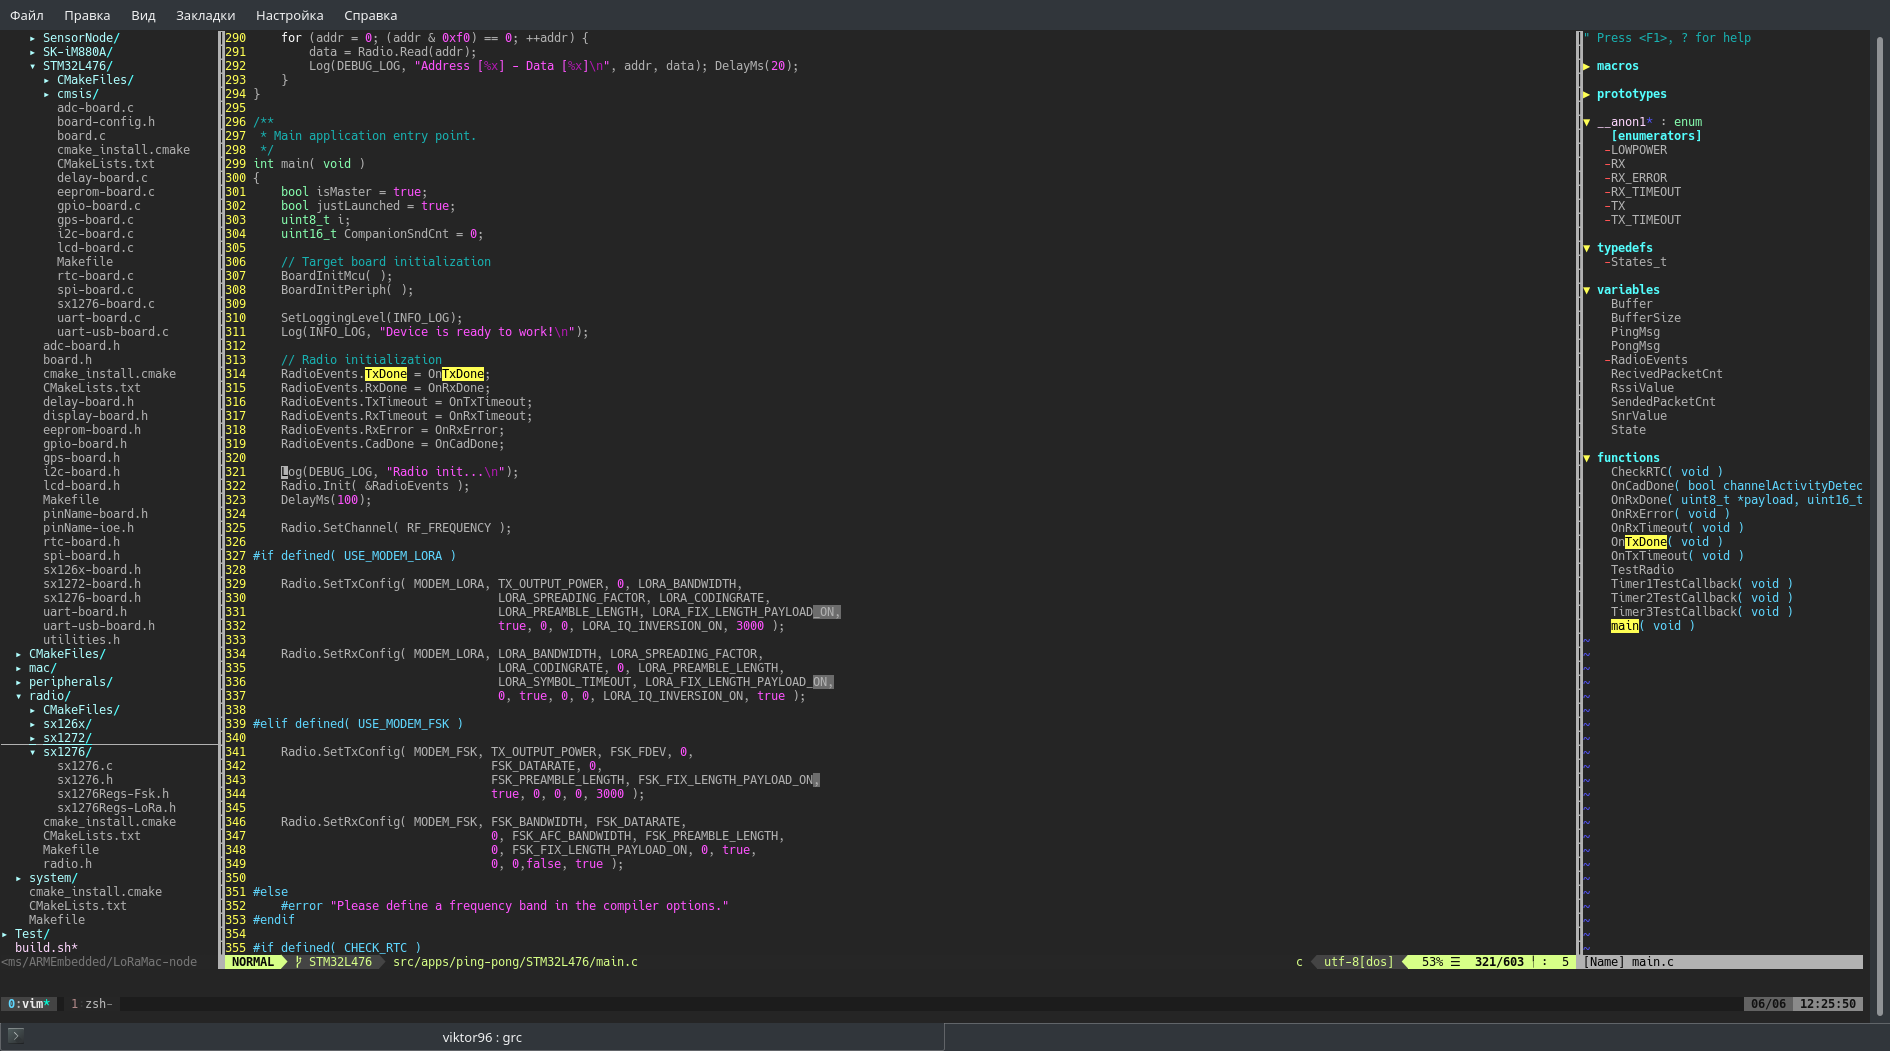
\includegraphics[width=\textwidth]{inc/img/Vim}
  \caption{Текстовый редактор Vim}
  \label{fig:ideeclipse}
\end{figure}

%+Зачем взял LoRaMac на гитхабе
%+Возможно немного слов про открытое ПО
%Ещё чуть чуть про инструменты

\subsubsection{CMake}

CMake ""--- это система сборки кроссплатформенного программного обеспечения из 
исходного кода. 
Она не занимается непосредственной сборкой, а лишь генерирует файлы управления 
сборкой исходя из инструкции в файле CMakeLists.txt.
Такими файлами управления сборкой могут служить файлы Makefile в системах Unix 
для сборки с помощью make, а также проекты XCode для Mac OS X и файлы 
project/solutions (\textit{.sln/.vcxproj/.vcproj}) в \textit{Windows} для 
сборки с помощью Visual C++.

CMake используется в выбранном проекте и пример файла CMakeLists.txt для сборки 
проектов под STM32L4 можно посмотреть в листинге \ref{lst:cmakestm32l4}.

\begin{listing}[H]
% firstline, lastline - какие строки показывать 
\cmakefile[lastline=11]{inc/src/stm32l4.cmake}
\caption{Инструкции для кросс-компиляции кода на платформу STM32L4 (часть 
файла)} 
\label{lst:cmakestm32l4}
\end{listing}

\subsubsection{HAL}

Для разработки программного обеспечения к аппаратной платформе STM32L476VGT6 
решено было использовать слой аппаратных абстракций (HAL), разработанный 
производителями микроконтроллеров семейства STM32 и распространяющийся на 
свободной основе.

HAL предоставляет возможность создания кода, не зависящего от аппаратных 
особенностей выбранной платформы. 
Хотя данный слой написан на языке Си, он реализует в себе множество идей 
объектно-ориентированного программирования (ООП). 
Самой важной идеей разработки такого программного обеспечения, как слой 
аппаратных абстракций, является инкапсуляция.
Инкапсуляция позволяет абстрагироваться от сложности разработки на низком 
уровне, предоставляя удобный интерфейс для написания программ работающих с 
различными устройствами, протоколами передачи данных и т.д.

%\subsection{Выбор компилятора для STM32}

%Раздел в процессе написания...

\subsubsection{ST-LINK/V2 и Openocd}

ST-LINK/V2 является внутрисхемным отладчиком и программатором для отладки 
микроконтроллеров семейства STM32 и STM8.
Данный отладчик спроектирован на базе микроконтроллера STM32F103C8, который 
включает в себя высокопроизводительное ядро ARM-Cortex M3.
Для внутрисхемной отладки он использует JTAG/SWD/SWIM интерфейсы отлаживаемого 
микроконтроллера.

ST-LINK/V2 уже входит в состав отладочной платы STM32L4-Discovery.

OpenOCD ""--- программное обеспечение для ОС Linux, Windows и Mac OS, 
реализующий интерфейс отлаживаемого микроконтроллера через внутрисхемный 
отладчик, такой как ST-LINK/V2 и другие. 
При запуске OpenOCD находит подключенный к компьютеру внутрисхемный отладчик, 
устанавливает с ним связь и открывает локальный TCP сервер, для последующего 
подключения к нему программного отладчика. 
TCP сервер OpenOCD принимает команды от программного отладчика и отсылает их 
внутрисхемному отладчику.
Инструкции подключения OpenOCD к внутрисхемному отладчику отображены в листинге 
\ref{lst:openocdconf}.

\begin{listing}[H]
% firstline, lastline - какие строки показывать 
\textfile{inc/src/openocd.cfg}
\caption{Инструкции подключения OpenOCD к внутрисхемному отладчику} 
\label{lst:openocdconf}
\end{listing}

В качестве программного отладчика была использована утилита arm-none-eabi-gdb, 
конфигурации для подключения можно увидеть в листинге \ref{lst:gdbconf}.

\begin{listing}[H]
% firstline, lastline - какие строки показывать 
\textfile{inc/src/gdb.cfg}
\caption{Инструкции подключения программного отладчика gdb к серверу OpenOCD} 
\label{lst:gdbconf}
\end{listing}

\subsection{Структура проекта LoRaMac}

Код проекта LoRaMAC разбит на несколько пакетов, каждый из которых реализует 
самостоятельный компонент программного обеспечения устройства:
\begin{itemize}
 \item \textit{system} ""--- слой аппаратных абстракций ``система'', 
использующийся пакетами поддержки радиомодулей и алгоритмов MAC. Является 
интерфейсом к используемому аппаратному обеспечению.
 \item \textit{boards} ""--- содержит реализации интерфейса абстракции 
``система'' для каждого вида микроконтроллера;
 \item \textit{radio} ""--- пакет, содержащий интерфейс и реализацию алгоритмов 
и данных для работы с приёмопередатчиками LoRa такими, как SX1272, SX1276, 
SX126x и другими. Для своей работы этот пакет использует слой аппаратных 
абстракции ``система''. 
 \item \textit{mac} ""--- пакет, реализующий данные и алгоритмы работы 
протокола LoRaWAN, включая шифрование данных и регионально-зависимые настройки 
несущих частот и прочих настроек физического уровня LoRa;
 \item \textit{apps} ""--- примеры готовых приложений;
 \item \textit{peripherals} ""--- различные драйверы для периферии, доступной 
на некоторых аппаратных платформах.
\end{itemize}

Упрощенную структуру проекта можно посмотреть на рисунке 
\ref{fig:loramacstructure}.

%Правила переноса кода
\begin{figure}[!h]
  \centering
  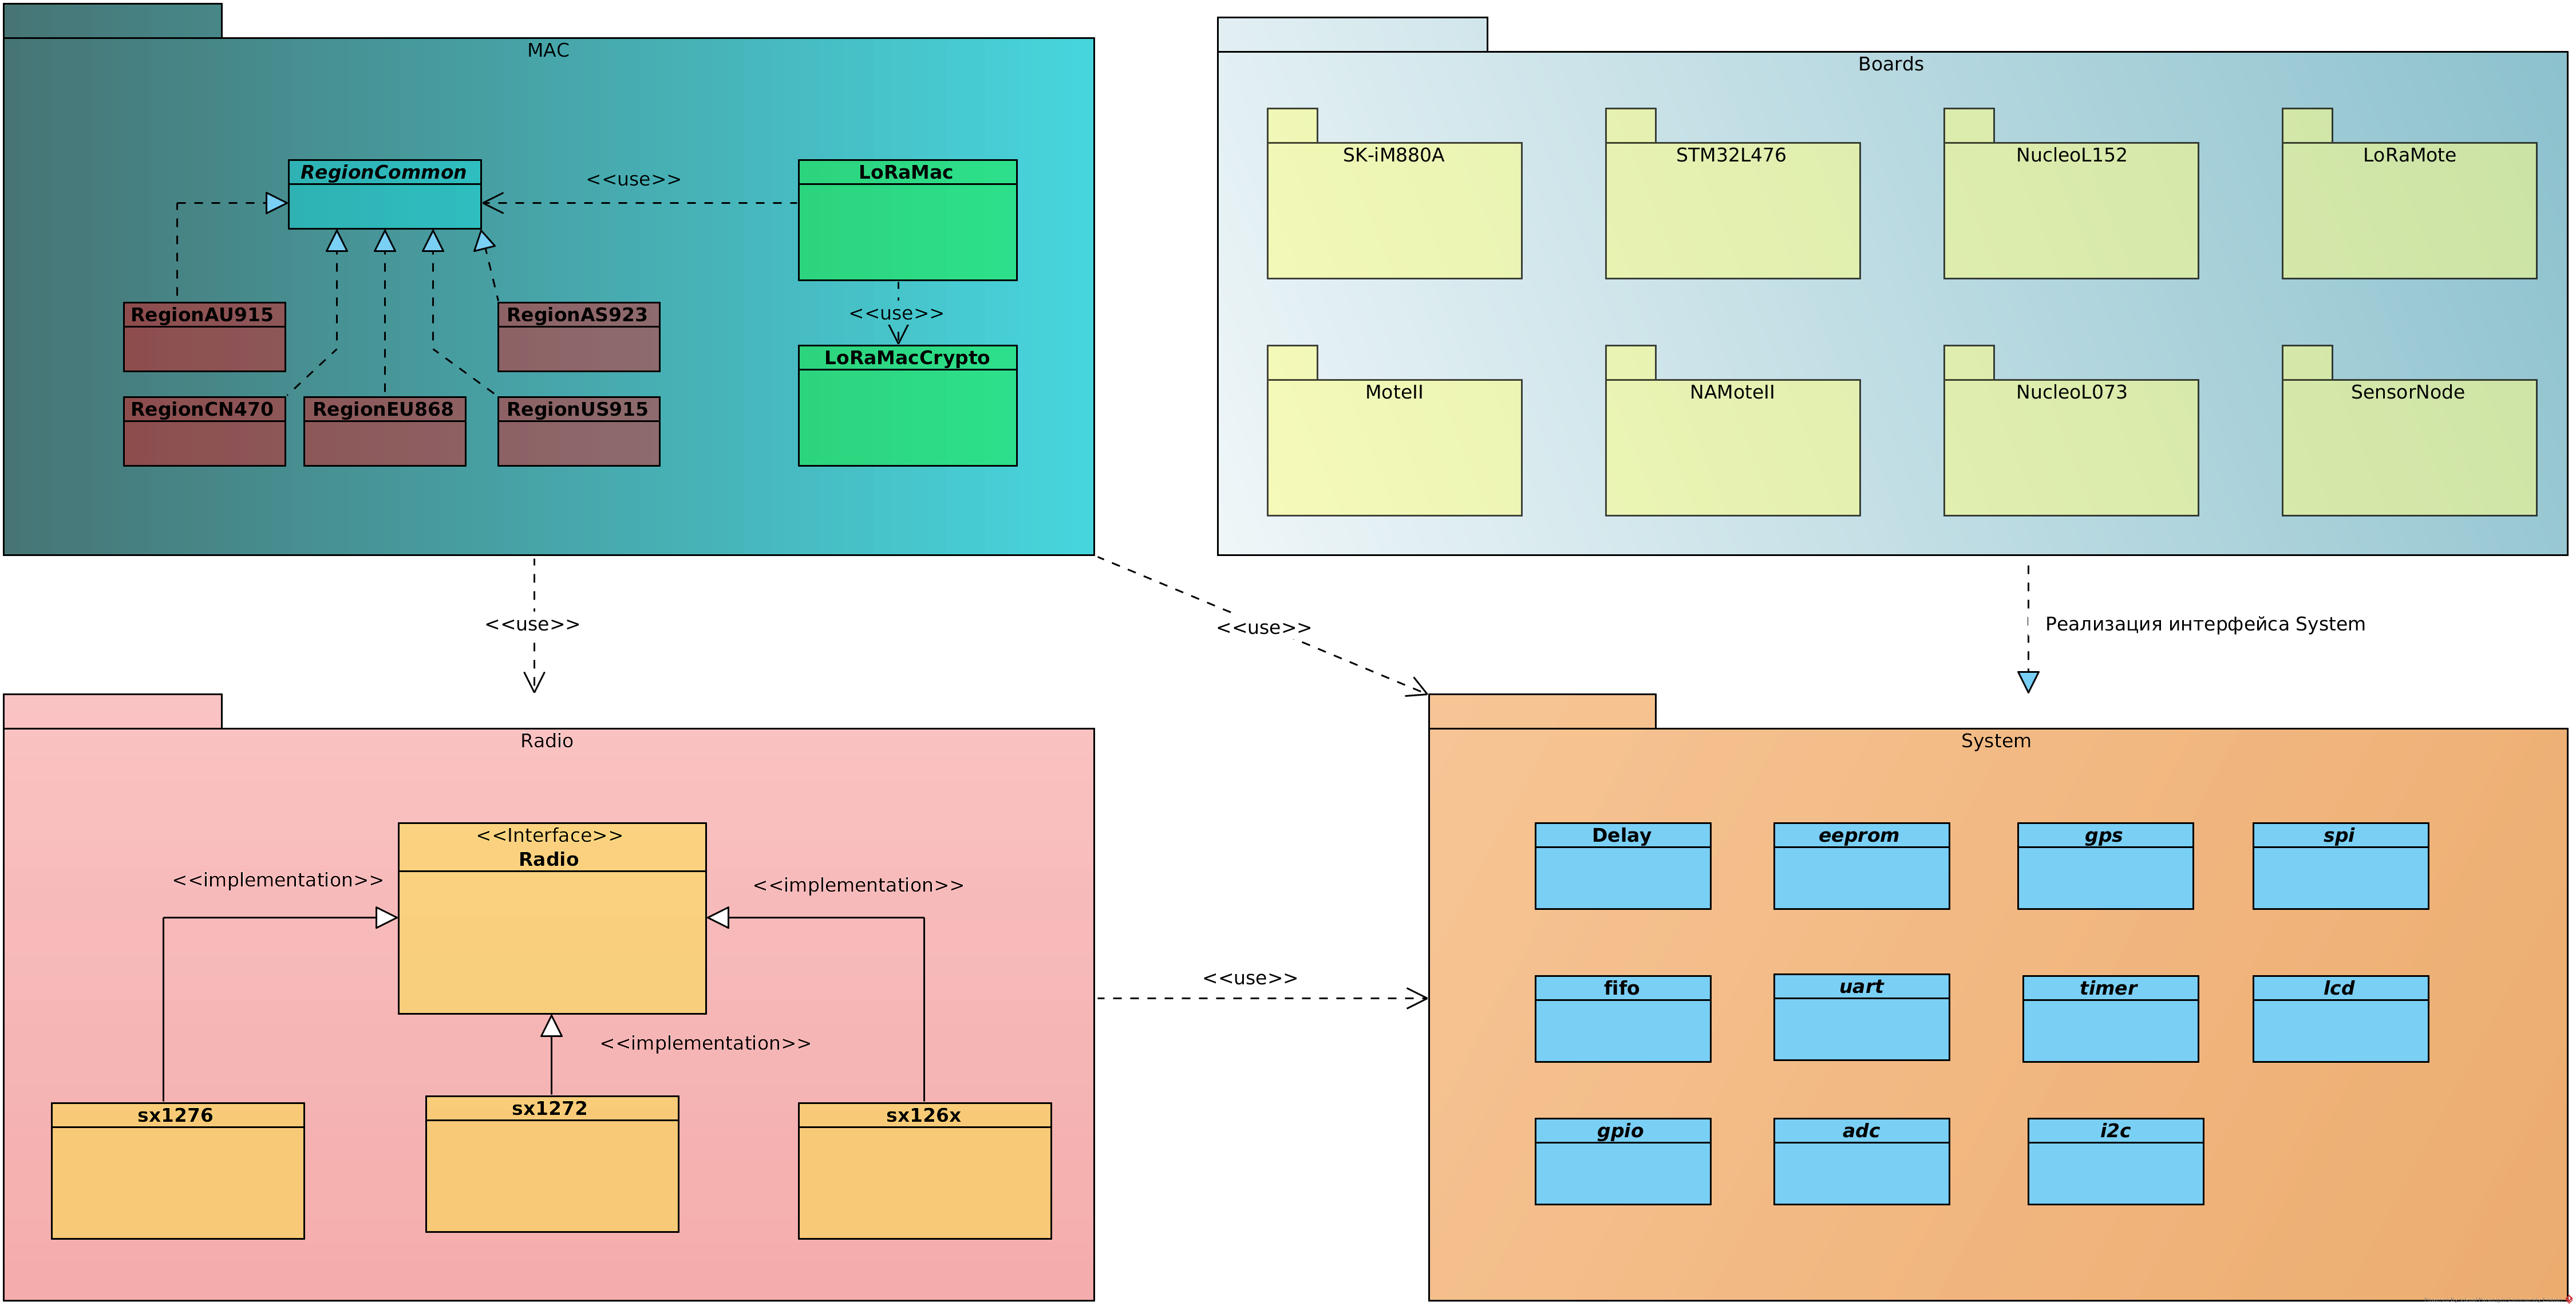
\includegraphics[width=\textwidth]{inc/img/LoRaMacProj}
  \caption{Упрощенная структура проекта LoRaMAC в нотации UML}
  \label{fig:loramacstructure}
\end{figure}

\section{Реализация проекта}

Проект LoRaMAC не содержал в себе исходного кода для реализации связки 
микроконтроллера STM32L476VGT6 на базе ядра ARM Cortex-M4, таким образом 
следовало сперва создать правила компиляции исходного кода для данной 
архитектуры. Эти правила описаны в файле \textit{stm32l4.cmake} и сам файл 
размещён в папке cmake в корне проекта. Часть содержимого этого файла 
отображено на листинге \ref{lst:cmakestm32l4}.

Как можно видеть из листинга, требуется также файл с инструкциями для 
компоновщика под выбранную аппаратную платформу. Код для компоновщика 
поставляется разработчиком аппаратных абстракции HAL.

Далее необходимо:
\begin{enumerate}
 \item добавить новую директорию в пакет \textit{boards} с именем используемой 
аппаратной платформы;
 \item реализовать интерфейс ``системы'' описав следующие модули под 
используемую аппаратную платформу:
 \begin{enumerate}
  \item board.c/.h;
  \item gpio-board.c/.h;
  \item piName-board.c/.h;
  \item piName-ioe.c/.h;
  \item rtc-board.c/.h;
  \item spi-board.c/.h.
 \end{enumerate}
 \item перенести в boards/mcu проект с HAL для STM32L4;
 \item занести конфигурацию оборудования в файл board-config.h.
\end{enumerate}

\subsection{Подключение STM32 к трансиверам LoRa}

Отладочная плата была соединена к интерфейсу SPI пирёмопередатчика SX1278.
Соответствие ножек и их функции приведено в таблице \ref{tab:stm32connect}.

\begin{table}[ht]
 \caption{Соответствие ножек отладочной платы и выполняемой функции}
\begin{tabular}{|c|c|}
\hline
\begin{tabular}[c]{@{}c@{}}Ножка отладочной \\ платы STM32L-DISCO\end{tabular} & 
\begin{tabular}[c]{@{}c@{}}Ножка радиомодуля\\ SX1278\end{tabular} \\ \hline
PE12                                                                           & 
NSS                                                                \\ \hline
PE13                                                                           & 
SCK                                                                \\ \hline
PE14                                                                           & 
MISO                                                               \\ \hline
PE15                                                                           & 
MOSI                                                               \\ \hline
PA5                                                                            & 
DIO0                                                               \\ \hline
PA1                                                                            & 
DIO1                                                               \\ \hline
PA2                                                                            & 
DIO2                                                               \\ \hline
PA3                                                                            & 
DIO3                                                               \\ \hline
PE11                                                                           & 
DIO4                                                               \\ \hline
PE10                                                                           & 
DIO5                                                               \\ \hline
PB7                                                                            & 
RESET                                                              \\ \hline
\end{tabular}
 \label{tab:stm32connect}
\end{table}

Собранный прототип отображен на рисунке \ref{fig:stm32lora}.

\begin{figure}[!h]
  \centering
  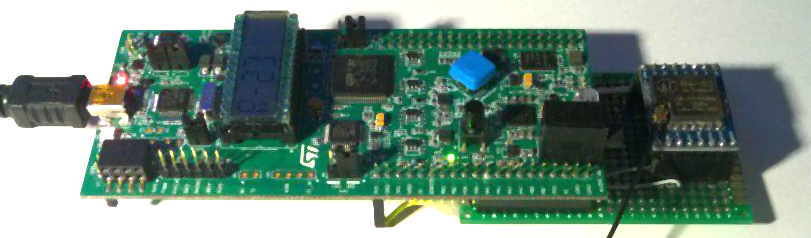
\includegraphics[width=\textwidth]{inc/img/stm32lora}
  \caption{Собранный прототип конечного устройства}
  \label{fig:stm32lora}
\end{figure}
% Желательно схему

\subsection{Сложности переноса}

Во время переноса кода на новую аппаратную платформу пришлось разрешить 
некоторые проблемы.
Во-первых, слой аппаратных абстракции не рассматривает использование новой
архитектуры ARM Cortex-M4, приходилось подбирать верные ключи для 
кросс-компиляции. 
Во-вторых, также не предполагалось использование SX1278, поэтому пришлось 
перенастроить частотные используемые частотные диапазоны в исходных файлах.
В-третьих, сам слой аппаратных абстракции содержит ошибки (неточности) в 
выбранных типах данных для интерфейсов.
Поскольку эти типы данных основаны на HAL, а HAL сам меняется, то в слое 
аппаратных абстракций LoRaMAC возникают множество неприятных ловушек, связанных 
с использование старой версии HAL.

Приведу конкретный пример: во время инициализации интерфейса SPI вызывалась 
функция выбора формата сигнала SPI ""--- \texttt{SpiFormat}:

\begin{minted}[linenos,breaklines,frame=single]{c}
if( nss == NC )
{
    SpiHandle[spiId].Init.NSS = SPI_NSS_SOFT;
    SpiFormat( obj, SPI_DATASIZE_8BIT, SPI_POLARITY_LOW, SPI_PHASE_1EDGE, 0 );
}
else
{
    SpiFormat( obj, SPI_DATASIZE_8BIT, SPI_POLARITY_LOW, SPI_PHASE_1EDGE, 1 );
}
\end{minted}

Второй параметр определяет сколько бит данных должен передавать один кадр SPI 
(в момент времени когда на линии \textit{NSS} логическая единица).
Готовый интерфейс аппаратных абстракций содержит следующее определение:
\begin{minted}[linenos,breaklines,frame=single]{c}
 /*!
 * \brief Configures the SPI peripheral
 *
 * \remark Slave mode isn't currently handled
 *
 * \param [IN] obj   SPI object
 * \param [IN] bits  Number of bits to be used. [8 or 16]
 * \param [IN] cpol  Clock polarity
 * \param [IN] cpha  Clock phase
 * \param [IN] slave When set the peripheral acts in slave mode
 */
void SpiFormat( Spi_t *obj, int8_t bits, int8_t cpol, int8_t cpha, int8_t slave 
);
\end{minted}

Здесь второй параметр определен как 8-битное целое число. 
Видимо первоначально предполагалось что туда будет передаваться всего два 
возможных значения ""--- \texttt{SPI\_DATASIZE\_8BIT} и 
\texttt{SPI\_DATASIZE\_16BIT}.
Так оно и было в старой версии HAL, однако в новой версии HAL для STM32L4 
добавились новые значения:

\begin{minted}[linenos,breaklines,frame=single]{c}
/** @defgroup SPI_Data_Size SPI Data Size            
  * @{                                               
  */                                                 
#define SPI_DATASIZE_4BIT               (0x00000300U)
#define SPI_DATASIZE_5BIT               (0x00000400U)
#define SPI_DATASIZE_6BIT               (0x00000500U)
#define SPI_DATASIZE_7BIT               (0x00000600U)
#define SPI_DATASIZE_8BIT               (0x00000700U)
#define SPI_DATASIZE_9BIT               (0x00000800U)
#define SPI_DATASIZE_10BIT              (0x00000900U)
#define SPI_DATASIZE_11BIT              (0x00000A00U)
#define SPI_DATASIZE_12BIT              (0x00000B00U)
#define SPI_DATASIZE_13BIT              (0x00000C00U)
#define SPI_DATASIZE_14BIT              (0x00000D00U)
#define SPI_DATASIZE_15BIT              (0x00000E00U)
#define SPI_DATASIZE_16BIT              (0x00000F00U)
\end{minted}

Как можно видеть теперь младший байт для передачи значения не используется, что 
приводило к неоднозначной ошибке исполнения программы: программа продолжала 
выполнятся, а SPI передавал 16 бит вместо 8. 
Ушло примерно два часа на анализ пока ошибка не была найдена и теперь 
определение функции выглядит так:

\begin{minted}[linenos,breaklines,frame=single]{c}
void SpiFormat( Spi_t *obj, int32_t bits, int8_t cpol, int8_t cpha, int8_t 
slave 
);
\end{minted}

Ошибка была исправлена. 
Безусловно подобные ошибки происходят не только по вине человека, но и по 
несовершенству средств программирования.
Язык Си является языком с, так называемой, мягкой типизацией, которая позволяет 
таким ошибкам происходить совершенно незаметно для разработчика.


%\begin{listing}[H]
% firstline, lastline - какие строки показывать 
%\cfile{inc/src/test.c}
%\caption{Пример — test.c} 
%\end{listing}
%\label{lst:c}

%Можно также использовать окружение \Code{verbatim}, если \Code{listings} чем-то не
%устраивает. Только следует помнить, что табы в нём <<съедаются>>. Существует так же команда \Code{\textbackslash{}verbatiminput} для вставки файла.

%\begin{verbatim}
%a_b = a + b; // русский комментарий
%if (a_b > 0)
    %a_b = 0;
%\end{verbatim}

%%% Local Variables:
%%% mode: latex
%%% TeX-master: "rpz"
%%% End:
